\documentclass[8pt]{extarticle}
\title{Econ 250 HW 10}
\author{Avinash Iyer}
\date{November 30, 2022}

%font setup
%
%\usepackage[math]{anttor}

%paper setup
\usepackage{geometry}
\geometry{letterpaper, portrait, margin=1in}
\usepackage{fancyhdr}

%symbols
\usepackage{amsmath}
\usepackage{amssymb}
\usepackage{hyperref}
\usepackage{gensymb}

\usepackage[T1]{fontenc}
\usepackage[utf8]{inputenc}

%chemistry stuff
\usepackage[version=4]{mhchem}
\usepackage{chemfig}

%plotting
\usepackage{pgfplots}
\usepackage{tikz}

%\usepackage{natbib}

%graphics stuff
\usepackage{graphicx}
\graphicspath{ {./images/} }

%a useful command
\newcommand{\plain}[1]{\textrm{#1}}

%code stuff
%when using minted, make sure to add the -shell-escape flag
%you can use lstlisting if you don't want to use minted
%\usepackage{minted}
%\usemintedstyle{pastie}
%\newminted[javacode]{java}{frame=lines,framesep=2mm,linenos=true,fontsize=\footnotesize,tabsize=3,autogobble,}
%\newminted[cppcode]{cpp}{frame=lines,framesep=2mm,linenos=true,fontsize=\footnotesize,tabsize=3,autogobble,}

\usepackage{listings}
\usepackage{color}
\definecolor{dkgreen}{rgb}{0,0.6,0}
\definecolor{gray}{rgb}{0.5,0.5,0.5}
\definecolor{mauve}{rgb}{0.58,0,0.82}

\lstset{frame=tb,
	language=Java,
	aboveskip=3mm,
	belowskip=3mm,
	showstringspaces=false,
	columns=flexible,
	basicstyle={\small\ttfamily},
	numbers=none,
	numberstyle=\tiny\color{gray},
	keywordstyle=\color{blue},
	commentstyle=\color{dkgreen},
	stringstyle=\color{mauve},
	breaklines=true,
	breakatwhitespace=true,
	tabsize=3
}
\pagestyle{fancy}
\fancyhf{}
\rhead{Avinash Iyer}
\lhead{Econ 250 HW 10}
\begin{document}{
\section*{Marginal Revenue and Elasticity}
\subsection*{Part A}
Clive is facing an inelastic demand curve as decreasing his price by 10\% only increases his quantity by 6.66\%, while Delia is facing an elastic demand curve as decreasing her price by 2\% increases her quantity by $6.66\%$.
\subsection*{Part B}
The marginal revenue for Clive is $\$4.50$, while the marginal revenue for Delia is $\$4.90$.
\subsection*{Part C}
A more inelastic demand indicates that the marginal revenue must decrease faster than a more elastic demand, as in the former case, a seller is facing consumers who are less sensitive to price decreases or increases
\section*{Monopoly, Standard Case}
\subsection*{Part A}
\begin{align*}
	TC &= 25Q + 2Q^2\\
	MC &= 25 + 4Q\\
	Q_D &= 500-2P\\
	P &= 250-Q/2\\
	PQ &= 250Q-Q^2/2\\
	MR &= 250-Q \\
	MR &= MC\\
	250-Q &= 25+4Q\\
	Q &= 45\\
\end{align*}

\subsection*{Part B}
The Lerner Index is equal to $\frac{-1}{E_{d}}$, or $-\frac{dP}{dQ}\left(\frac{Q}{P}\right) = \frac{45}{205}$.
\subsection*{Part C}
We calculate the optimal quantity $Q^{*}$ by finding when $MC = D$, indicating that our result is $Q^{*} = 50$. The value of $P - MC$ at the market quantity is $22.5$, so our final deadweight loss is $(1/2)(22.5)(5) = 56.25$.
\section*{Monopolies versus Perfectly Competitive Firms}
\begin{center}
	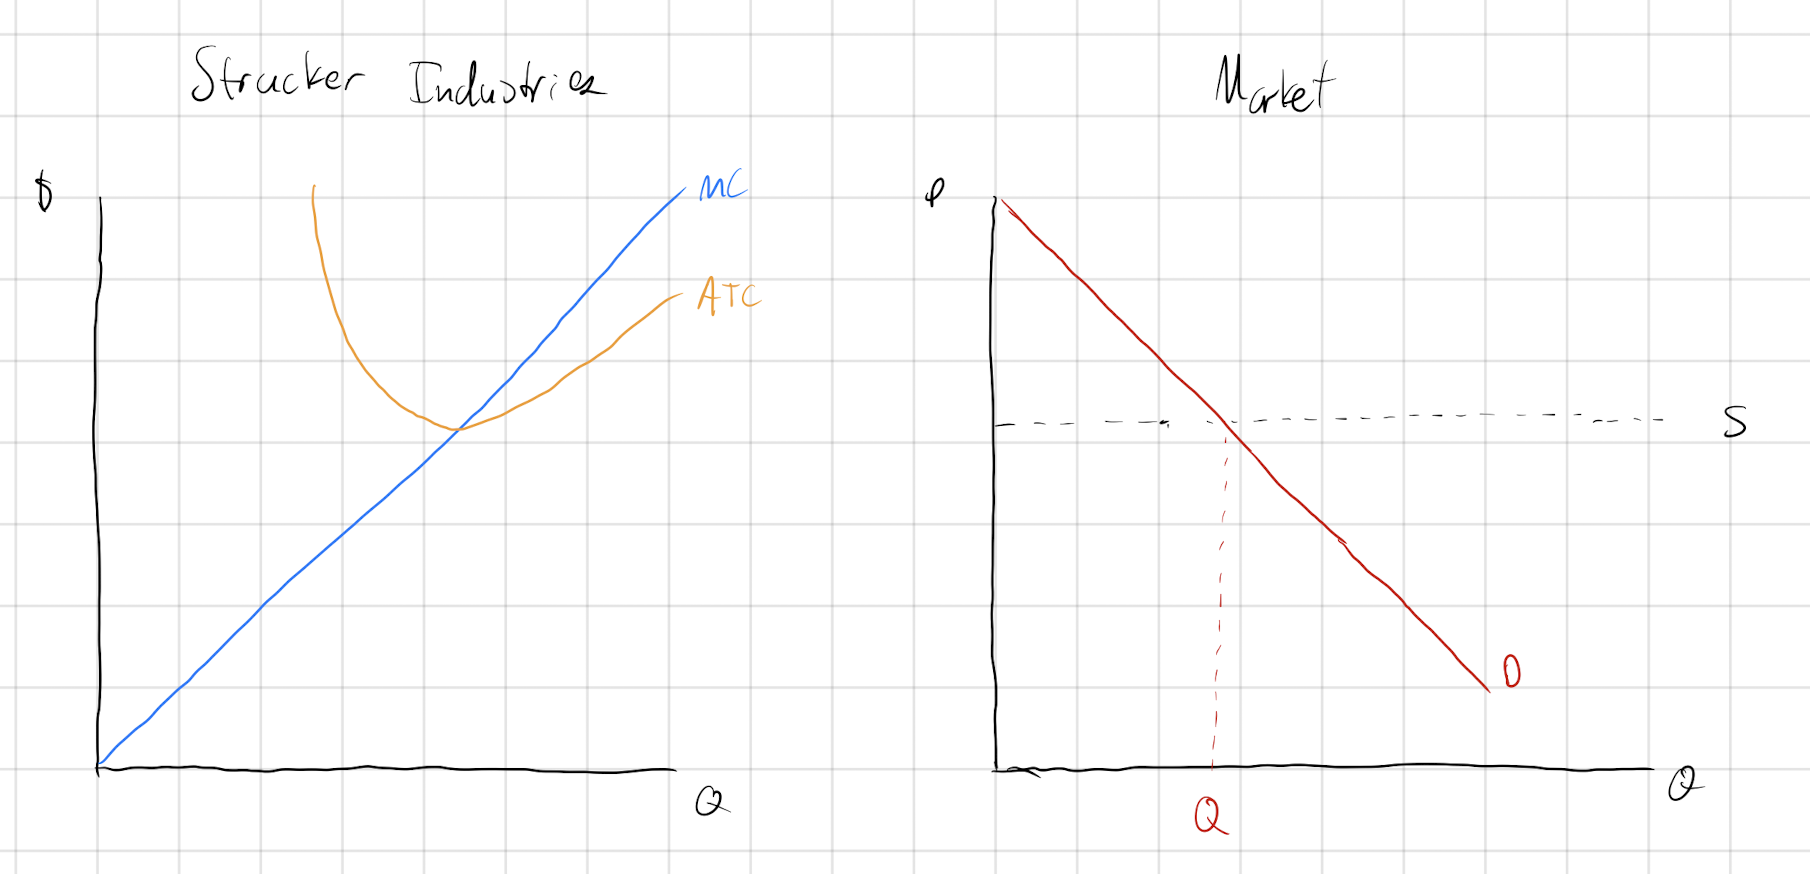
\includegraphics[width=10cm]{HW10Q3A}\\
	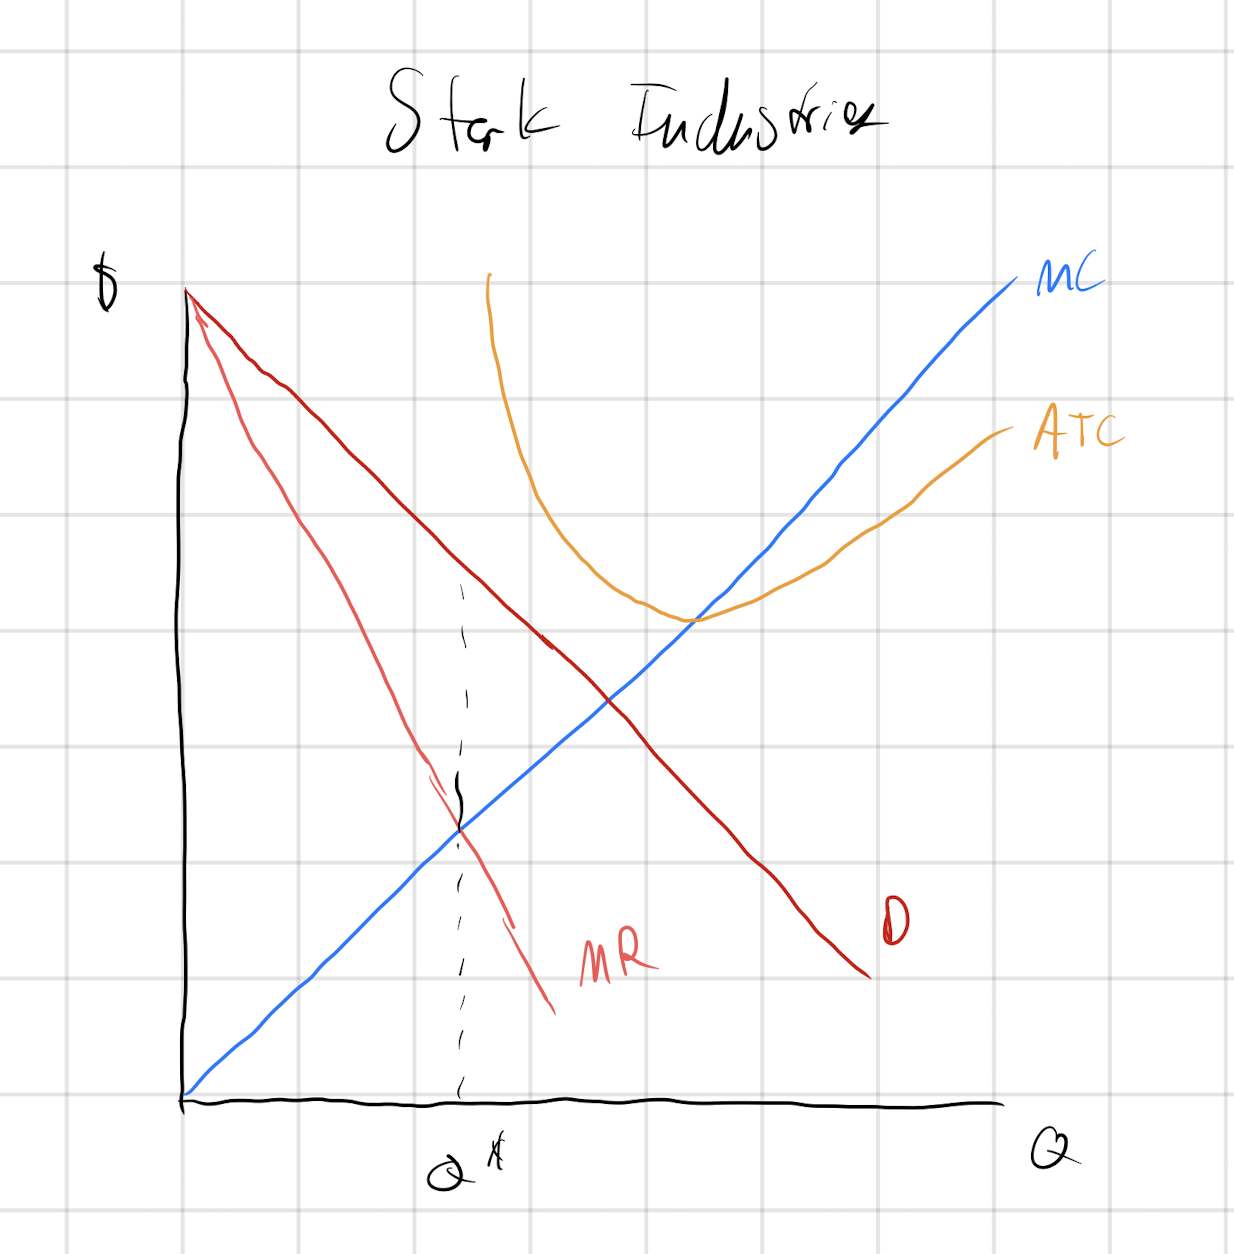
\includegraphics[width=10cm]{HW10Q3B}
\end{center}
Since the $MR$ curve for the monopolist Stark industries is always below the demand curve for Stark industries, the quantity produced will always be \textbf{lower} than in perfect competition (assuming no ability for price discrimination).
\section*{Monopolies and Taxes}
\begin{center}
	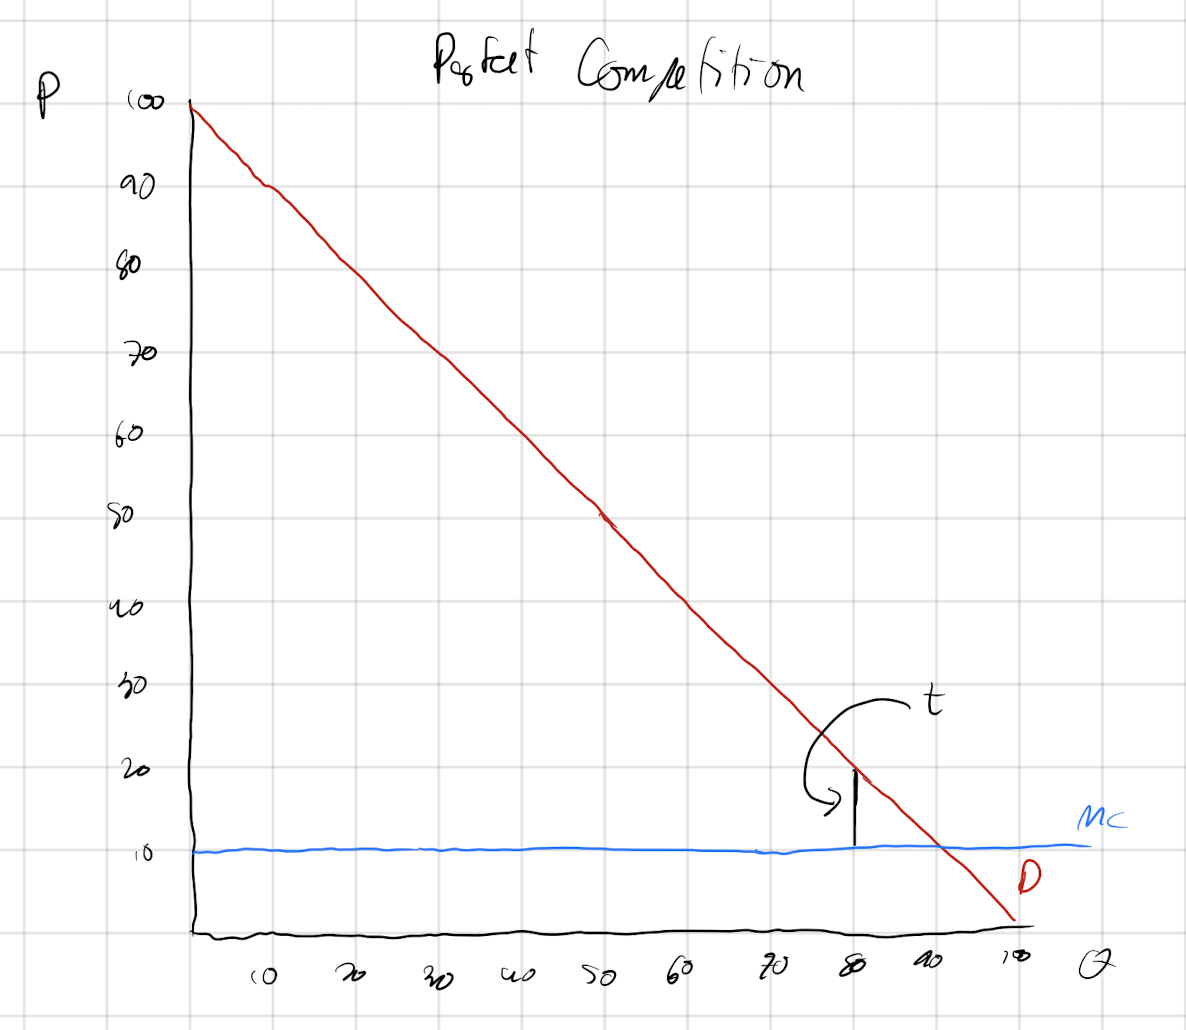
\includegraphics[width=10cm]{HW10Q4A}\\
	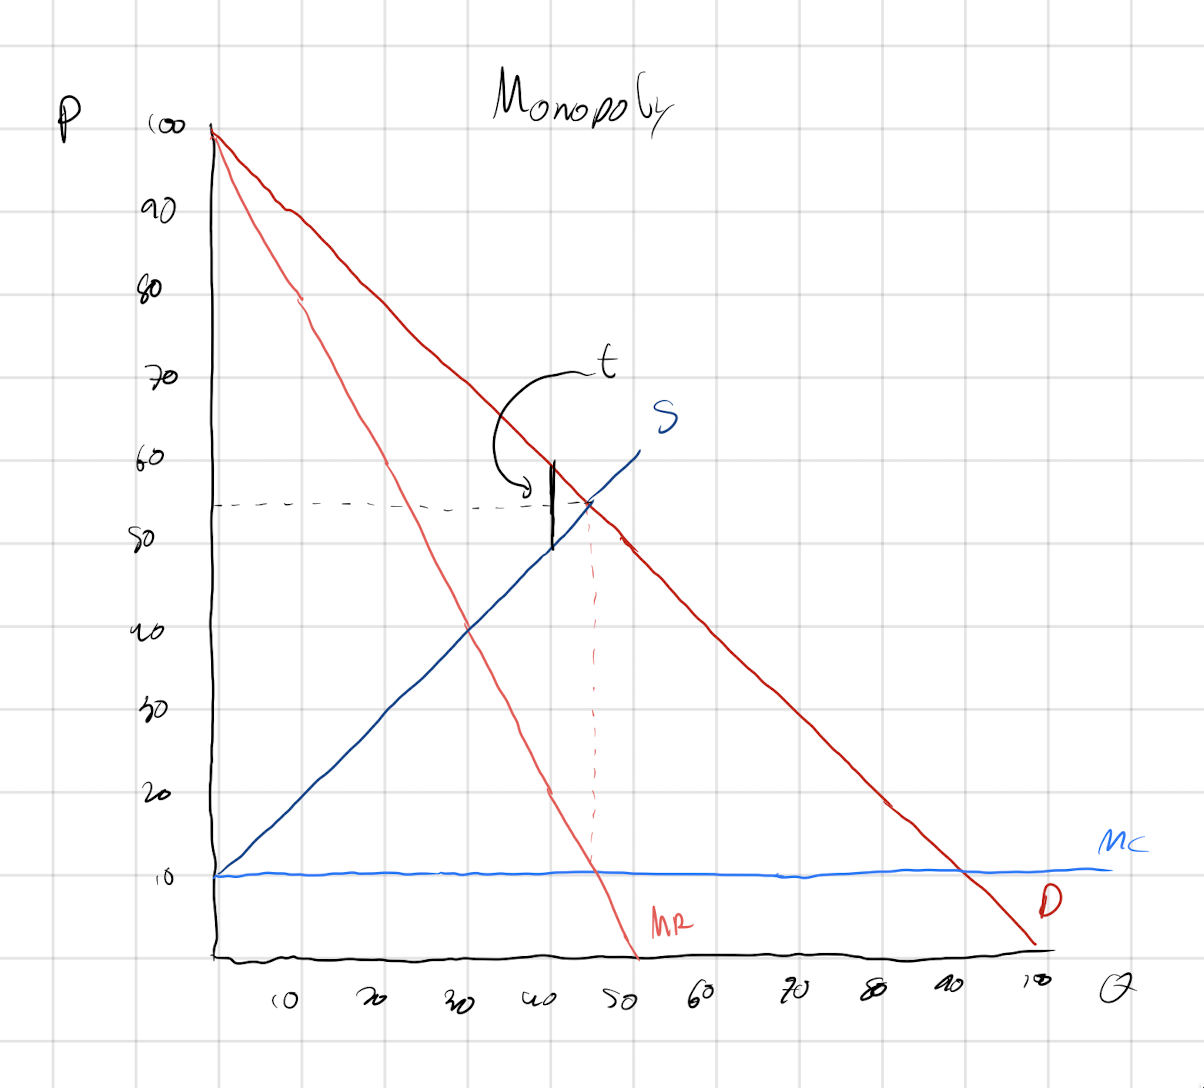
\includegraphics[width=10cm]{HW10Q4B}
\end{center}
As seen in the above graphs, the tax incidence falls entirely on consumers in perfect competition while the tax incidence is split between consumers and producers in monopoly.
\section*{Monopolies with Fixed Costs}
\subsection*{Part A}
The firm \textbf{is} a natural monopoly as the demand curve intersects $LATC$ while $LATC$ is downward sloping, indicating that any firms entering the market would face high fixed costs while expanding production within an existing firm would have lower average costs.
\subsection*{Part B}
The firm \textbf{will} earn a profit if it is not subject to regulation since price the firm charges at the quantity where marginal revenue equals marginal cost is higher than the $LATC$ curve.
\subsection*{Part C}
If the firm mandates that the firm charge no more than the marginal cost, the firm will have to charge $\$10$, which is below the average total cost at $Q = 1000$, meaning the firm will be driven out of business.
\subsection*{Part D}
The firm will sell 700 units at $\$25$ if the price is capped at average total costs. However, this quantity is not the optimal quantity of $1000$.
\subsection*{Part E}
\begin{center}
	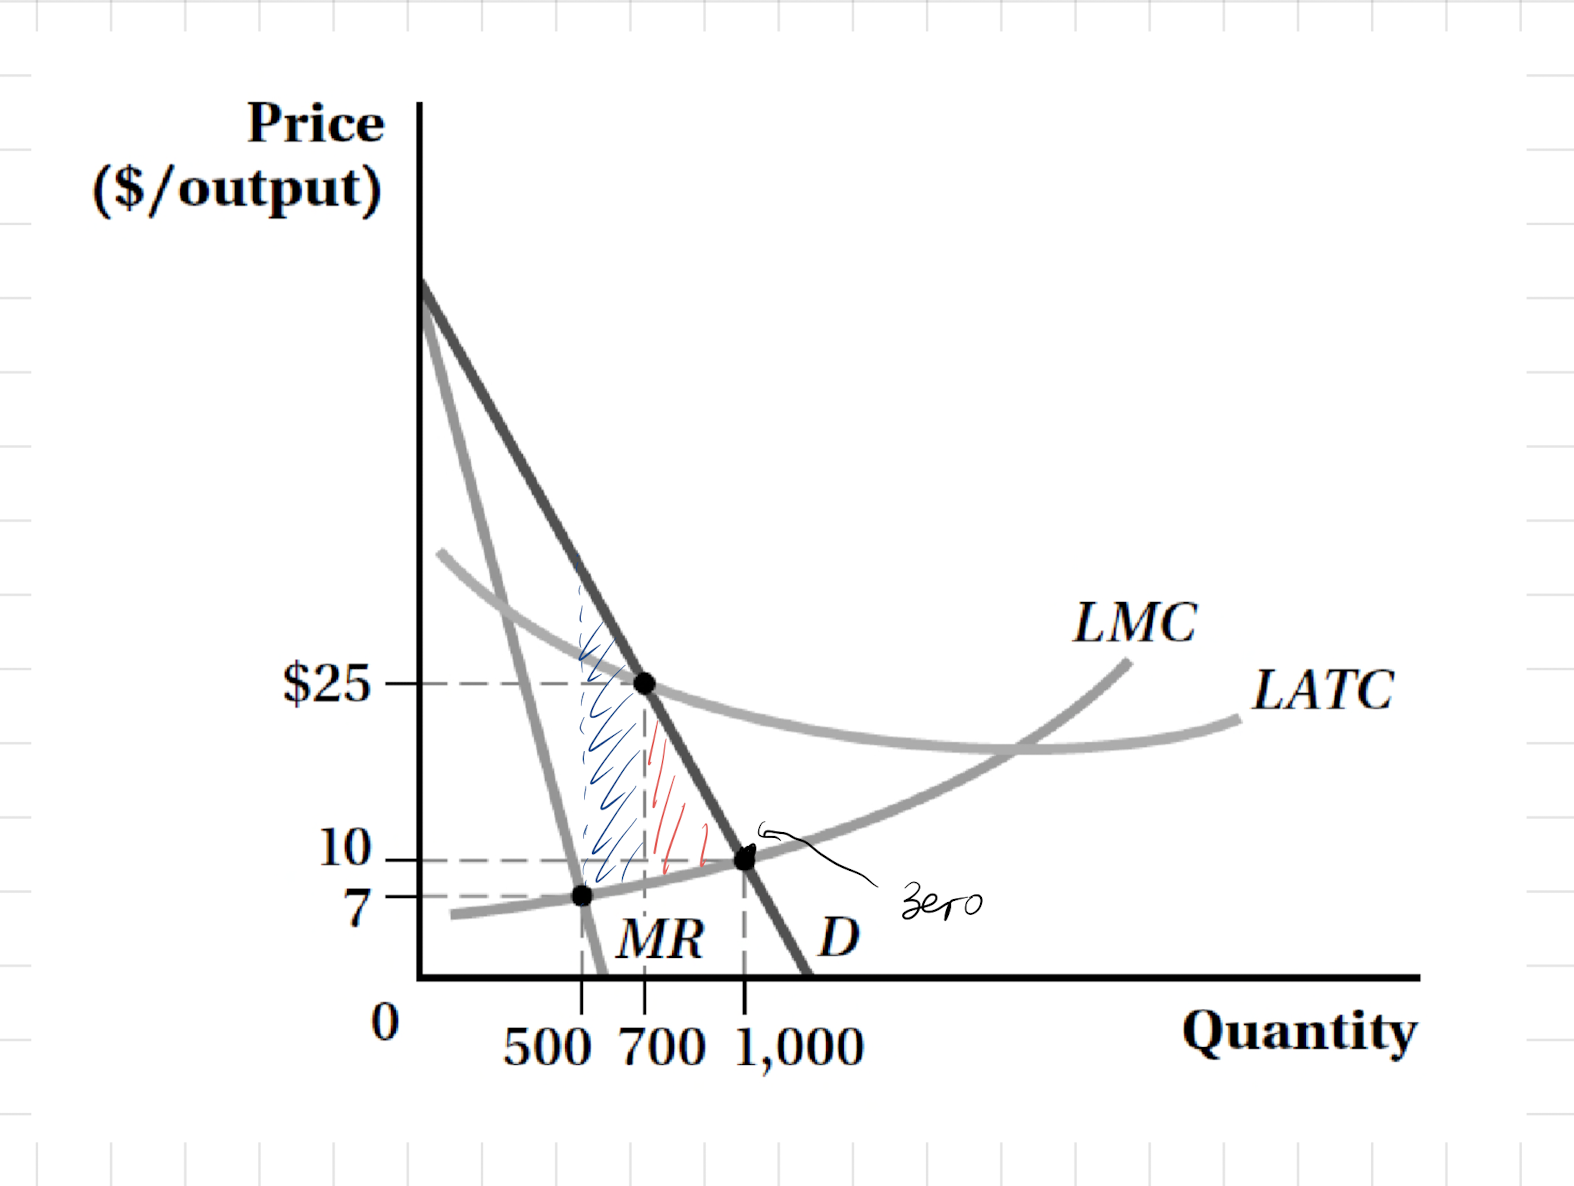
\includegraphics[width=10cm]{HW10Q5E}
\end{center}
The DWL in the case of Part B will be equal to the Blue + Red segments, the case of Part C will be zero, and the case of Part D will be equal to the Red segment.
\section*{Price Discrimination, Conceptually}
\begin{itemize}
	\item There is deadweight loss compared to competitive equilibriume because the marginal revenue is still below demand for the various segments that the firm sets out.
	\item The company should offer a discount to consumers in Area B --- since demand in Area B is highly inelastic, the marginal revenue curve is very steep, meaning that the quantity of tutoring services provided in the area is very close to the optimal quantity. Providing a discount in Area B would thus have very little effect on the total quantity of tutoring services provided compared to providing a discount in Area A.
\end{itemize}
\section*{Perfect Price Discrimination, Operation Decisions}
\begin{align*}
	Q &= 200 - P\\
	P &= 200-Q\\
	MR &= 200-Q\\
	TC &= 10000 + \frac{1}{3}Q^2\\
	MC &= \frac{2}{3}Q\\
	ATC &= 10000/Q + \frac{1}{3}Q\\
	MC &= MR\\
	\frac{2}{3}Q &= 200-Q\\
	Q &= 120\\
	P &= 80\\
	ATC &= 123.33
\end{align*}
Since $ATC$ is higher than $P$, Cogsworth will \textbf{shut down} in the long run.
\section*{Perfect Price Discrimination, Inferring Marginal Cost}
\begin{align*}
	TC &= 100 + mQ\\
	ATC &= 100/Q + m\\
	MC &= m\\
  P &= 20-Q/5\\
  MR &= 20-Q/5\\
  20-Q/5 &= m\\
  Q &= 100-5m\\
  \pi &= TR - TC\\
      &= TR - TVC - TFC\\
      &= (PS) - 100\\
  390 &= PS - 100\\
  PS &= 490\\
  \frac{1}{2}(100-5m)(20-m) &= 490\\
  980 &= 5(20-m)^2\\
  196 &= 20-m\\
  m &= 6
\end{align*}
\section*{First Degree Price Discrimination, Different Consumers}
\subsection*{Part A}
\begin{center}
	\begin{tabular}{c|c|c}
	Quantity & Price & Marginal Revenue\\
	\hline
	1 & 7 & 7\\
	2 & 6 & 5\\
	3 & 5 & 3\\
	4 & 4 & 1\\
	\end{tabular}
\end{center}
As seen in the table above, the marginal revenue hits the marginal cost at $3.5$ Butterfingers, meaning that we will provide 3 butterfingers and set price to $5$. This means that total costs are $6$ and total revenue is $15$, for a profit of $9$. On the diagram, we see that setting the price to $5$ creates a deadweight loss of $3$ from the three consumers unable to buy the butterfingers. Meanwhile, the consumer surplus is also $3$ as seen from the diagram.
\subsection*{Part B}
We will sell butterfingers up to the marginal consumer, meaning that we will sell up to Marge, or $6$ butterfingers. By adding up the various boxes on the diagram, we get a profit of $15$. Meanwhile, since we are selling the butterfingers at the customers' willingness to pay, their consumer surplus is zero, and we also have zero deadweight loss.
\subsection*{Part C}
Consumer surplus gets translated into producer surplus and profit as a result of the ability to perfectly price discriminate.
\subsection*{Part D}
Deadweight loss disappears as we are able to sell to all consumers willing to pay up to our marginal cost.
\section*{Third Degree Price Discrimination, Standard Case}%
  \begin{align*}
    Q_M &= 50 - 0.5P\\
    P_{M} &= 100-2Q\\
    MR &= 100-4Q\\
    TC &= 100Q\\
    MC &= 10\\
    MR &= MC\\
    100-4Q &= 10\\
    4Q &= 90\\
    Q &= 22.5\\
    \pi_1 &= (P-ATC)(Q)\\
        &= (100-2(22.5) - (10))(22.5)\\
        &= 1012.5
        \\
    Q_{O} &= 100-2P\\
    P &= 50-Q/2\\
    MR &= 50-Q\\
    MC &= 10\\
    MR &= MC\\
    50-Q &= 10\\
    Q &= 40\\
    \pi_2 &= (P-ATC)(Q)\\
          &= (50-(40/2)-10)(40)\\
          &= 800\\
          \\
    \pi &= \pi_1 + \pi_2\\
        &= \boxed{1812.5}
  \end{align*}
\section*{Third Degree Price Discrimination, Increasing Marginal Costs}%
\subsection*{Part A}%
  \begin{align*}
    Q_B &= 500-P\\
    P &= 500-Q_B\\
    MR_B &= 500-2Q_B\\
    500-2Q_B &= 2Q_B + 2Q_E\\
    \\
    Q_E &= 700-2P\\
    P &= 350-Q_E/2\\
    MR &= 350-Q_E\\
    350-Q_E &= 2Q_B + 2Q_E\\
    \\
    500-4Q_B &= 2Q_E\\
    Q_E &= 250-2Q_B\\
    350-(250-2Q_B) &= 2Q_B + 500-4Q_B\\
    100+2Q_B &= 500-2Q_B\\
    Q_B &= \boxed{100}\\
    Q_E &= 250-2(100)\\
    Q_E &= \boxed{50}
  \end{align*}
\subsection*{Part B}%
  United should charge $400$ for business class fliers and $325$ for economy class fliers. 

}\end{document}
